\clearpage
\onecolumn
\section{Exploratory Implanted-ICL Variable Pilot}

\subsection{Cohort, Models, and Validation}

This analysis was a separate exploratory pilot and was not pooled with the main v5 cohorts. It included 26 eyes from 14 patients (12 bilateral and 2 unilateral). The implanted-ICL input (ICL3) comprised size, power, and model. Seven frozen Ridge-based modality combinations were evaluated on the same cohort and splits.

The five prespecified repeat seeds were 42, 1001, 2002, 2026, and 3407. Each repeat used five-fold patient-grouped outer cross-validation, and each outer-training partition used three-fold patient-grouped inner cross-validation. Patient grouping was enforced at both levels, so eyes from the same patient could not be split across the corresponding inner-training/validation or outer-training/test partitions. Hyperparameters were selected solely by mean inner-validation eye-level MAE. Each model produced exactly one outer out-of-fold prediction per eye per repeat. No best repeat or post-hoc model was selected.

AS-OCT images underwent EXIF orientation correction, RGB conversion, direct resizing to $224 \times 224$ without cropping, conversion to $[0,1]$ tensors using ToTensor, and normalization with the ImageNet channel means $(0.485, 0.456, 0.406)$ and standard deviations $(0.229, 0.224, 0.225)$. An ImageNet-pretrained ResNet18 with all backbone parameters frozen supplied the 512-dimensional global-average-pooled penultimate representation. The encoder was neither fitted nor updated using outer-test data or labels.

Within each inner split, all continuous-feature scalers were fitted exclusively on the inner-training partition. The categorical ICL model was one-hot encoded fold-locally; unseen categories were ignored and represented by all-zero indicator vectors, with no ordinal integer encoding. PCA was used only for models containing AS-OCT and was fitted only on inner-training data, with candidate dimensions 2, 4, and 8. Ridge $\alpha$ candidates were 0.01, 0.1, 1, 10, 100, and 1000. Configurations were selected by mean inner-validation eye-level MAE; exact ties favored the larger $\alpha$ and then fewer PCA components. After selection, the complete pipeline was refitted only on the corresponding outer-training data and evaluated once on the outer-test fold. Outer-test data and labels did not participate in fitting scalers, PCA, categorical encoders, or Ridge models, or in hyperparameter selection.

The prespecified primary model combined AS-OCT, measurements, and ICL3; its comparator combined AS-OCT and measurements. Delta MAE was primary minus comparator, so negative values favored the primary model. The uncertainty analysis used the frozen 10,000-resample patient-clustered percentile bootstrap with seed 42. All findings are exploratory and not confirmatory.

\subsection{Model Performance and Primary Comparison}

\FloatBarrier

\begin{table}[H]
\centering
\caption{Seven frozen pilot models. Overall MAE is reported as mean $\pm$ SD across five repeats; High-vault MAE is the descriptive mean across five repeats. Numerical rankings are descriptive, and no unplanned pairwise inference was performed.}
\label{tab:supp_pilot_models}
\footnotesize
\setlength{\tabcolsep}{4pt}
\begin{tabular}{llrrrr}
\toprule
Model & Inputs & Eyes & Patients & MAE ($\mu$m) & High-vault MAE ($\mu$m) \\
\midrule
AS-OCT only & AS-OCT & 26 & 14 & $153.268 \pm 10.057$ & 213.173 \\
Measurement only & Measurement & 26 & 14 & $197.497 \pm 13.496$ & 242.380 \\
Comparator & AS-OCT + Measurement & 26 & 14 & $162.059 \pm 16.008$ & 215.335 \\
ICL3 only & ICL3 & 26 & 14 & $199.412 \pm 14.155$ & 269.280 \\
AS-OCT + ICL3 & AS-OCT + ICL3 & 26 & 14 & $170.567 \pm 14.223$ & 229.902 \\
Measurement + ICL3 & Measurement + ICL3 & 26 & 14 & $203.778 \pm 12.206$ & 251.160 \\
Primary & AS-OCT + Measurement + ICL3 & 26 & 14 & $160.859 \pm 18.568$ & 221.535 \\
\bottomrule
\end{tabular}
\end{table}

\begin{table}[H]
\centering
\caption{Prespecified primary paired comparison. The bootstrap interval crosses zero and is not an equivalence test.}
\label{tab:supp_pilot_primary}
\footnotesize
\setlength{\tabcolsep}{5pt}
\resizebox{\textwidth}{!}{%
\begin{tabular}{lrrrrrr}
\toprule
Contrast & Comparator MAE & Primary MAE & Mean delta & Bootstrap delta & 95\% CI & Improved/tied/worse \\
\midrule
Primary $-$ comparator & 162.059 & 160.859 & $-1.200$ & $-0.972$ & $[-10.941,\ 8.847]$ & 7/0/7 \\
\bottomrule
\end{tabular}
}
\end{table}

\begin{table}[H]
\centering
\caption{Patient-level mean paired absolute-error differences. Negative values favor the primary model. Patient identifiers are anonymized.}
\label{tab:supp_pilot_patients}
\footnotesize
\setlength{\tabcolsep}{5pt}
\begin{tabular}{lrrl@{\qquad}lrrl}
\toprule
Patient & Eyes & Delta ($\mu$m) & Category & Patient & Eyes & Delta ($\mu$m) & Category \\
\midrule
001 & 1 & 8.402 & Worse & 048 & 2 & 7.249 & Worse \\
008 & 2 & 19.266 & Worse & 051 & 2 & $-18.695$ & Improved \\
047 & 1 & $-4.432$ & Improved & 144 & 2 & $-9.124$ & Improved \\
145 & 2 & $-12.536$ & Improved & 146 & 2 & $-39.794$ & Improved \\
147 & 2 & 10.734 & Worse & 186 & 2 & 1.633 & Worse \\
187 & 2 & $-3.698$ & Improved & 188 & 2 & 15.320 & Worse \\
189 & 2 & $-25.125$ & Improved & 194 & 2 & 37.185 & Worse \\
\bottomrule
\end{tabular}
\end{table}

\begin{table}[H]
\centering
\caption{Repeat-level primary comparison. Negative delta favors the primary model.}
\label{tab:supp_pilot_repeats}
\footnotesize
\setlength{\tabcolsep}{4pt}
\begin{tabular}{rrrr}
\toprule
Seed & Eyes & Comparator MAE & Primary MAE / delta \\
\midrule
42 & 26 & 147.940 & 148.074 / 0.134 \\
1001 & 26 & 151.086 & 163.075 / 11.989 \\
2002 & 26 & 153.076 & 136.432 / $-16.644$ \\
2026 & 26 & 183.788 & 177.417 / $-6.371$ \\
3407 & 26 & 174.405 & 179.297 / 4.892 \\
\bottomrule
\end{tabular}
\end{table}

\begin{figure}[H]
\centering
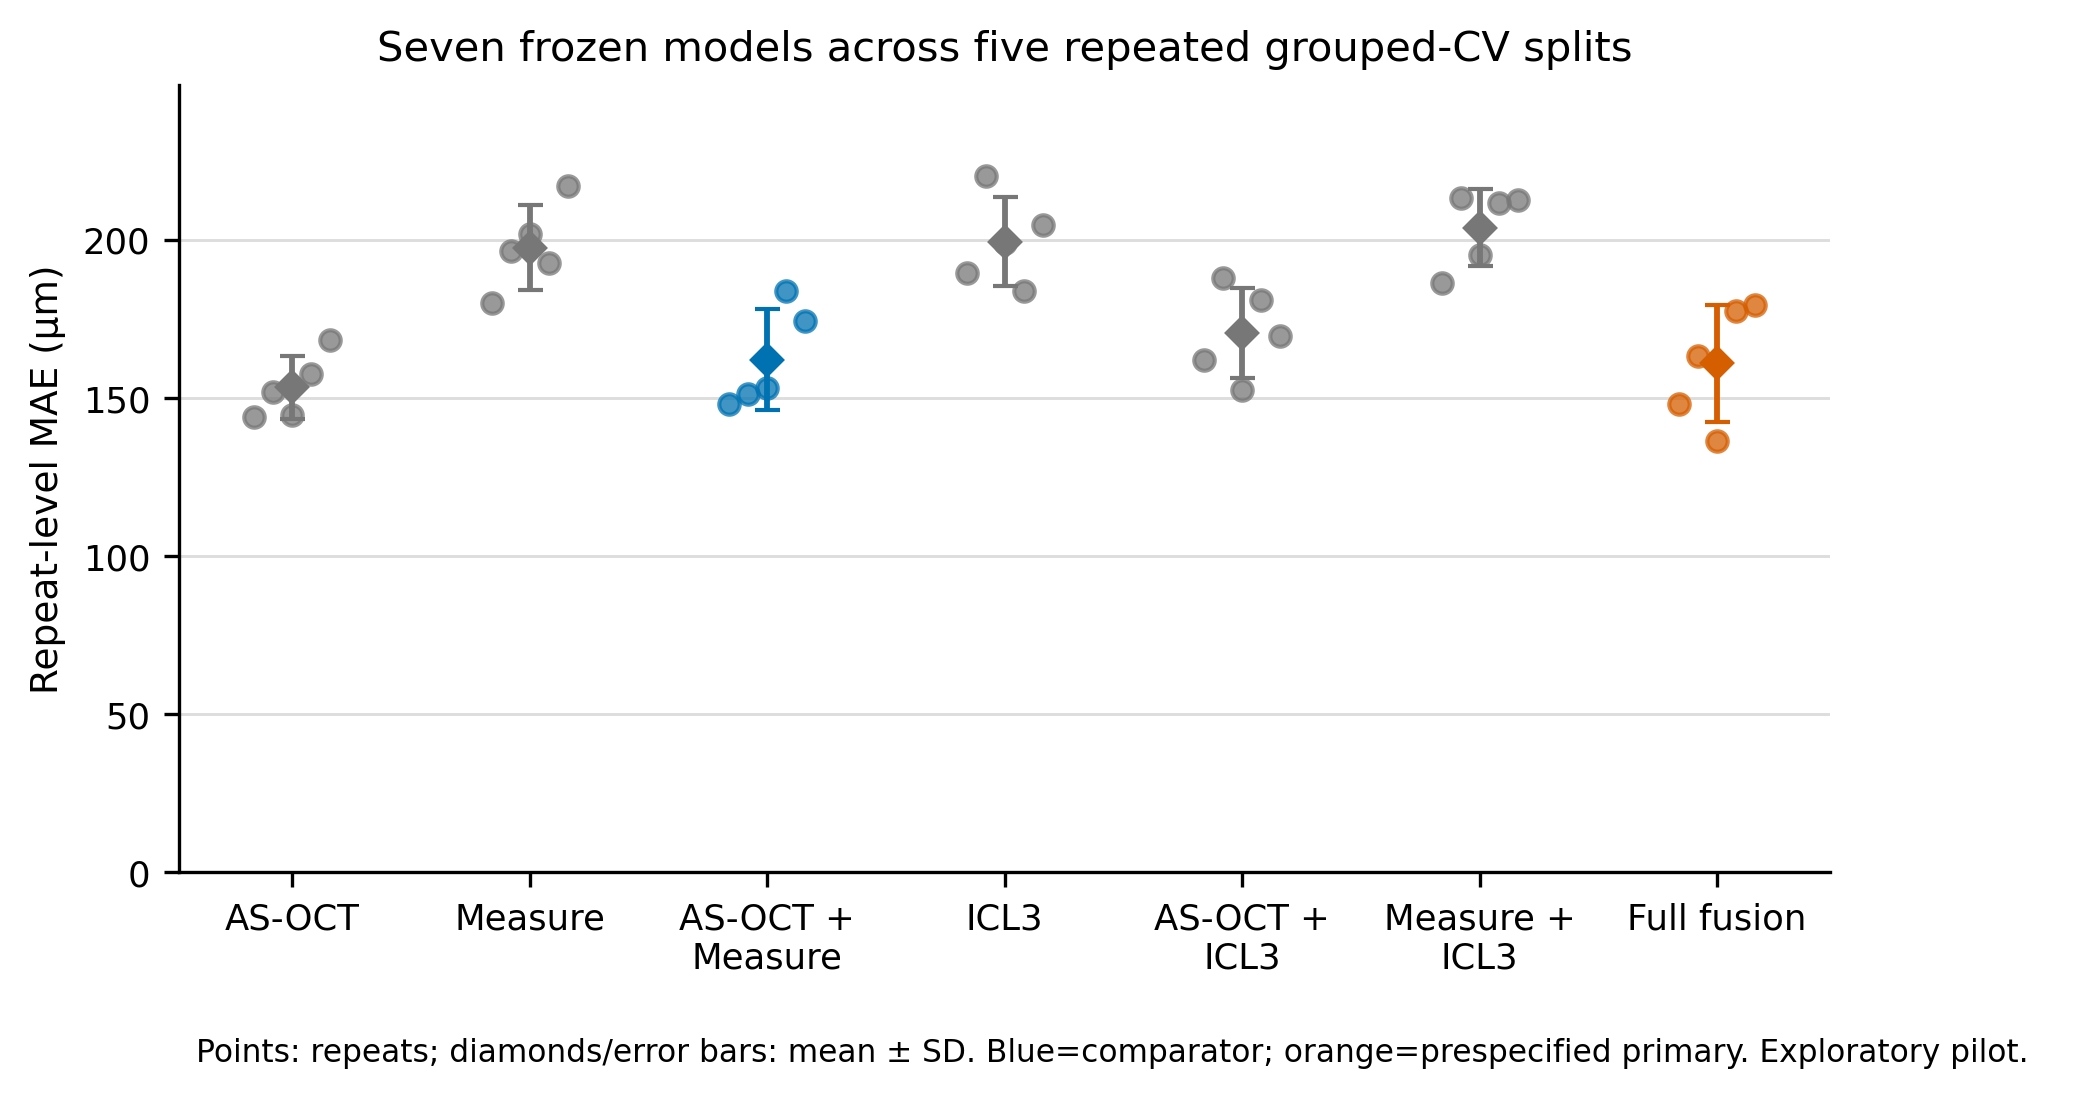
\includegraphics[width=0.88\textwidth]{figures/fig_supp_pilot_model_mae.png}
\caption{Descriptive MAE distributions for all seven frozen pilot models across five repeats. Numerical ranking does not imply inferential superiority.}
\label{fig:supp_pilot_model_mae}
\end{figure}

\begin{figure}[H]
\centering
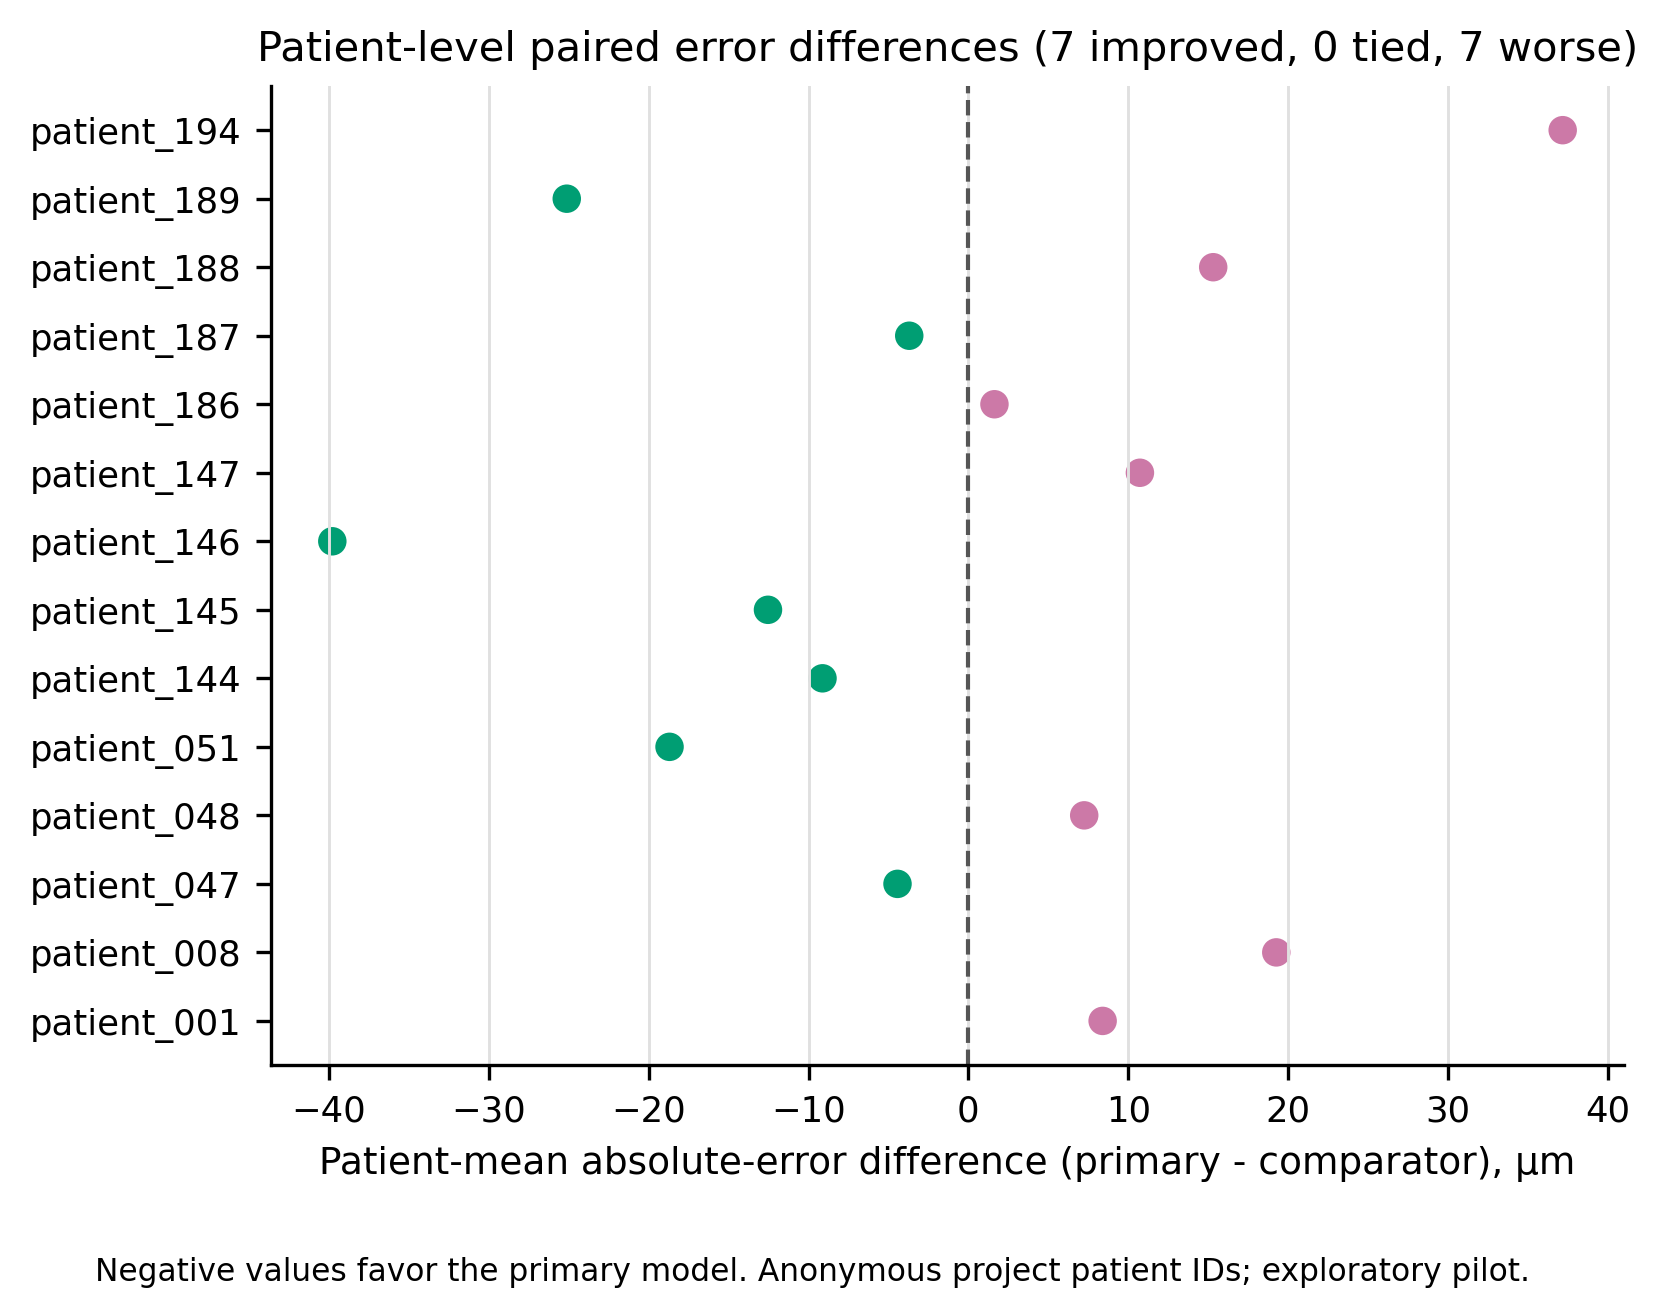
\includegraphics[width=0.78\textwidth]{figures/fig_supp_pilot_patient_delta.png}
\caption{Patient-level mean paired absolute-error differences for the primary model versus comparator. Negative values favor the primary model; 7 patients improved, none tied, and 7 worsened.}
\label{fig:supp_pilot_patient_delta}
\end{figure}

\FloatBarrier

\subsection{Outer-Fold Stability and Prediction Patterns}

\FloatBarrier

\begin{table}[H]
\centering
\caption{Outer-fold mean paired absolute-error differences in $\mu$m. Negative values favor the primary model. The number of paired eyes is shown in parentheses.}
\label{tab:supp_pilot_outer_folds}
\footnotesize
\setlength{\tabcolsep}{6pt}
\begin{tabular}{lrrrrr}
\toprule
Seed & Fold 0 & Fold 1 & Fold 2 & Fold 3 & Fold 4 \\
\midrule
42 & 49.176 (5) & $-0.327$ (5) & $-47.727$ (6) & 1.729 (4) & 6.447 (6) \\
1001 & 4.052 (6) & 0.754 (4) & 16.089 (6) & $-1.926$ (4) & 32.592 (6) \\
2002 & 0.068 (5) & $-0.529$ (5) & $-77.285$ (6) & 1.058 (4) & 4.840 (6) \\
2026 & 30.164 (5) & 0.739 (6) & $-1.159$ (6) & $-3.046$ (3) & $-50.803$ (6) \\
3407 & $-5.887$ (5) & $-2.299$ (6) & 2.245 (6) & 33.480 (5) & $-2.611$ (4) \\
\bottomrule
\end{tabular}
\end{table}

\begin{figure}[H]
\centering
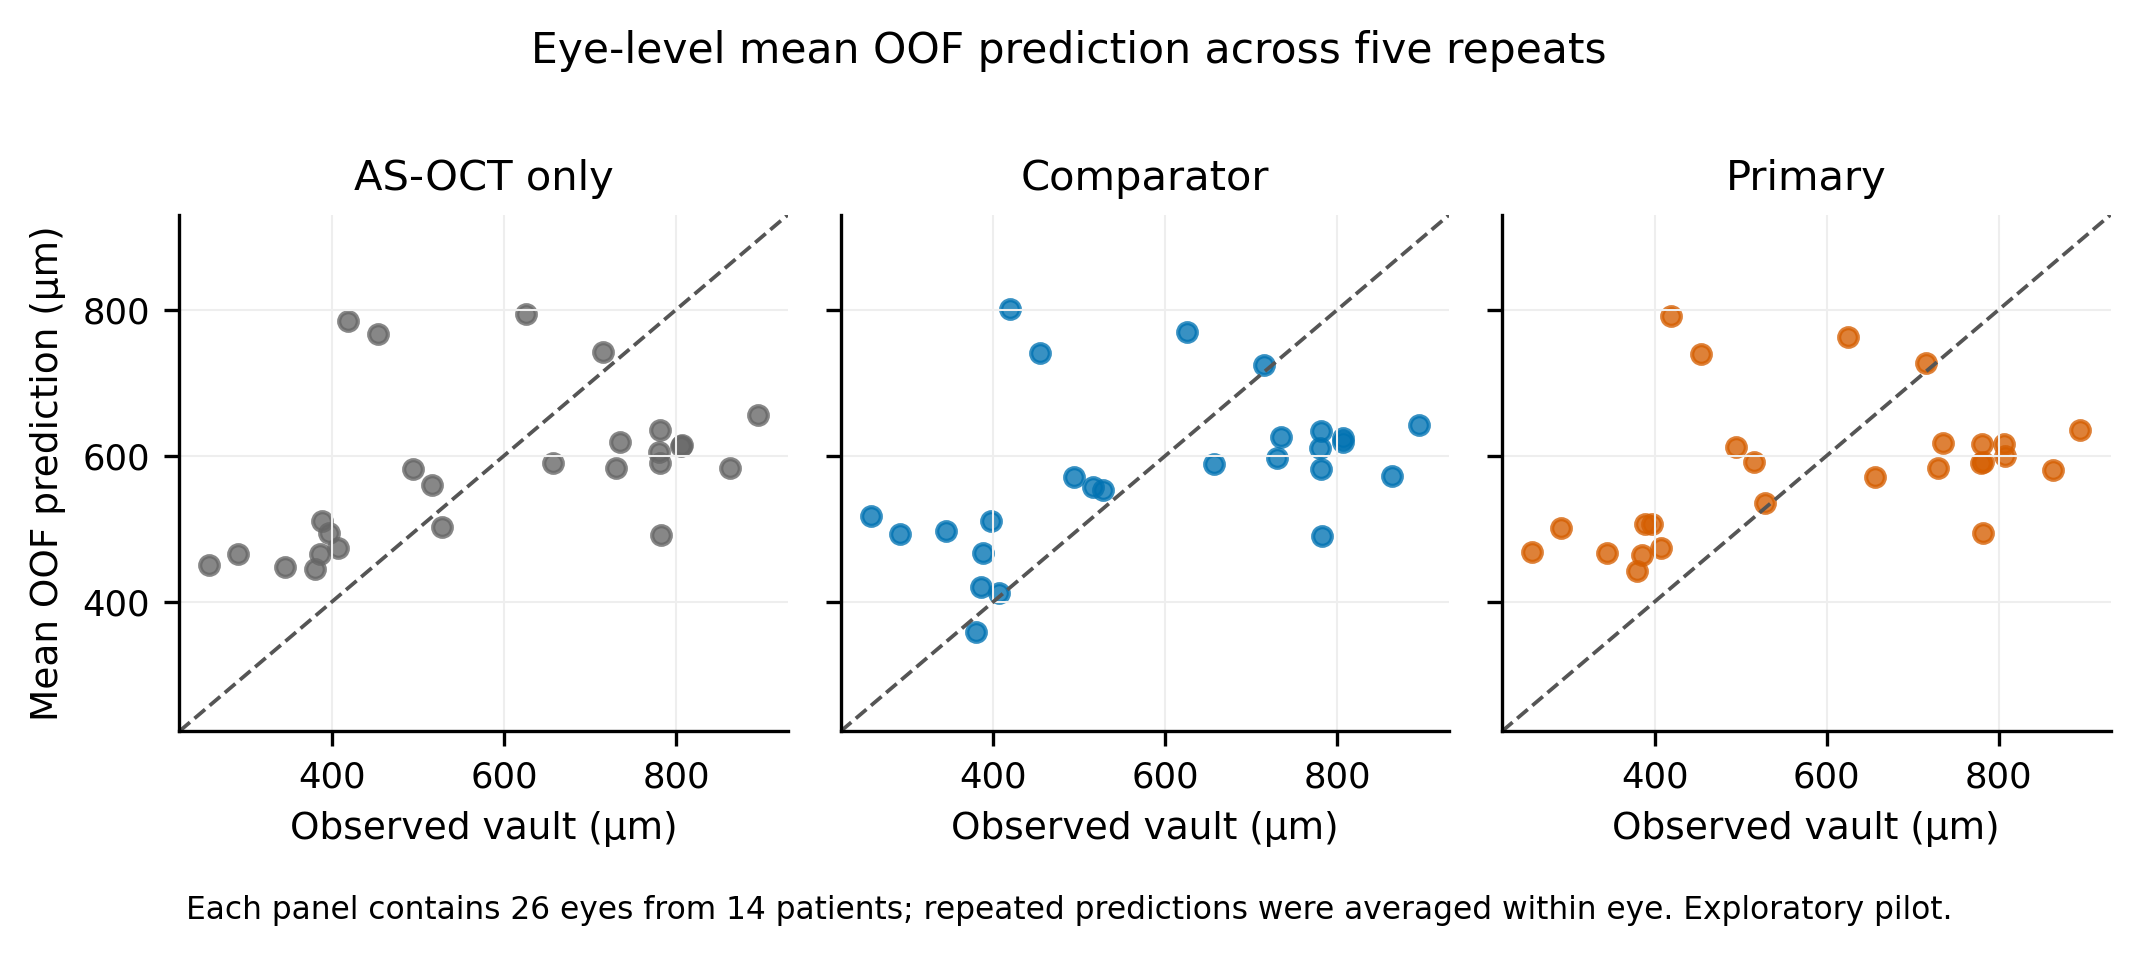
\includegraphics[width=0.94\textwidth]{figures/fig_supp_pilot_oof_scatter.png}
\caption{Eye-level mean out-of-fold predictions across five repeats for AS-OCT-only, comparator, and primary models. Each panel uses 26 eyes as display units; the 910 repeated model predictions are not treated as independent samples.}
\label{fig:supp_pilot_oof_scatter}
\end{figure}

\begin{figure}[H]
\centering
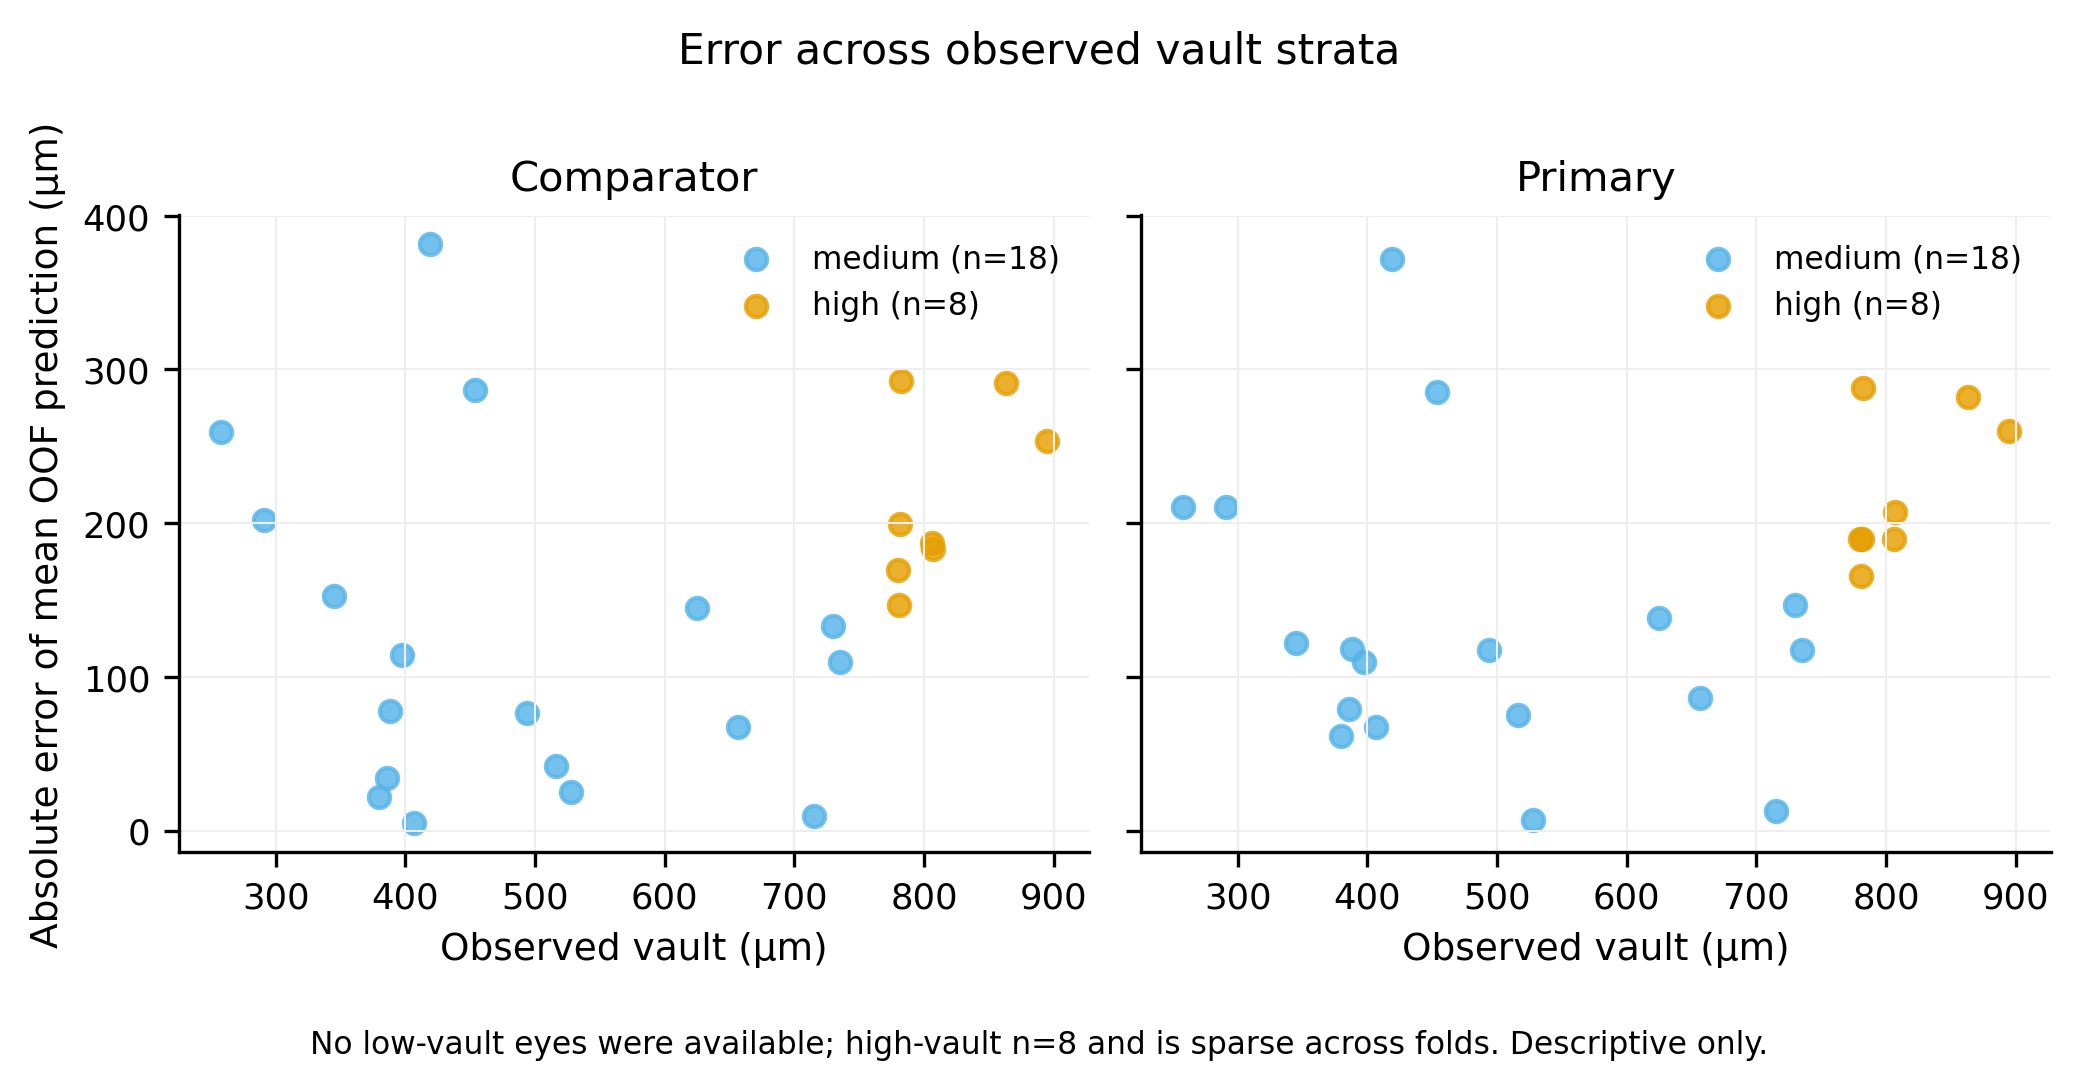
\includegraphics[width=0.90\textwidth]{figures/fig_supp_pilot_vault_error.png}
\caption{Descriptive error patterns by observed vault for the comparator and primary models. The cohort contained 18 medium-vault and 8 high-vault eyes and no low-vault eyes; no low-vault conclusion is available.}
\label{fig:supp_pilot_vault_error}
\end{figure}

\FloatBarrier

\subsection{Hyperparameter Selection Stability}

Hyperparameters were selected independently within each outer training analysis; no global hyperparameter was selected. The 25 selections per model were distributed as shown below. A pair denotes Ridge $\alpha$/PCA components; PCA was not applicable to models without AS-OCT. Categorical ICL model encoding was performed fold-locally.

\FloatBarrier

\begin{table}[H]
\centering
\caption{Fold/repeat hyperparameter selection frequencies. Counts sum to 25 within each model. These frequencies describe selection instability and do not define a global setting.}
\label{tab:supp_pilot_hyperparameters}
\scriptsize
\setlength{\tabcolsep}{3pt}
\begin{tabular}{lp{0.78\textwidth}}
\toprule
Model & Selected $\alpha$/PCA combinations (count) \\
\midrule
AS-OCT only & 0.01/2 (4), 0.01/8 (14), 10/8 (1), 100/2 (1), 100/4 (3), 1000/2 (1), 1000/4 (1) \\
Measurement only & 0.1/NA (1), 1/NA (2), 10/NA (5), 100/NA (9), 1000/NA (8) \\
Comparator & 0.1/4 (1), 10/4 (3), 10/8 (7), 100/2 (2), 100/4 (1), 100/8 (8), 1000/2 (1), 1000/4 (2) \\
ICL3 only & 0.1/NA (1), 1/NA (2), 10/NA (15), 100/NA (2), 1000/NA (5) \\
AS-OCT + ICL3 & 0.01/4 (1), 0.1/8 (1), 1/2 (1), 1/4 (1), 10/2 (1), 10/4 (2), 10/8 (3), 100/2 (2), 100/4 (1), 100/8 (11), 1000/4 (1) \\
Measurement + ICL3 & 0.1/NA (1), 10/NA (5), 100/NA (12), 1000/NA (7) \\
Primary & 10/8 (5), 100/2 (4), 100/4 (1), 100/8 (12), 1000/2 (1), 1000/4 (2) \\
\bottomrule
\end{tabular}
\end{table}

\FloatBarrier

\subsection{Coverage, Integrity, and Reporting Scope}

The cohort contained 18 medium-vault and 8 high-vault eyes and no low-vault eyes. Nine outer folds and eight inner folds contained no high-vault sample, so range-specific findings are descriptive. All 25 evaluations were complete with zero detected patient-leakage failures. The locked closure preserved 2,250 hyperparameter-configuration identities and 6,750 inner-fit scope records. Raw inner-fold predictions and MAE values were not persisted and were not reconstructed. The pilot lacks external validation and cannot support confirmatory, equivalence, absolute-null, or external-generalization claims.

\FloatBarrier
